% latex table generated in R 2.15.3 by xtable 1.7-1 package
% Mon Apr 28 15:44:10 2014
\begin{table*}[ht]
\centering
\begin{tabular}{rp{27em}rrrrc}
  \hline
Feature & Description & quant\_5 & mean & median & quant\_95 & histogram \\ 
  \hline
   \multicolumn{2}{l}{\bfseries{Java}}  \\
all & All issues recorded for the project. & 1.00 & 23.37 & 3.00 & 80.00 & 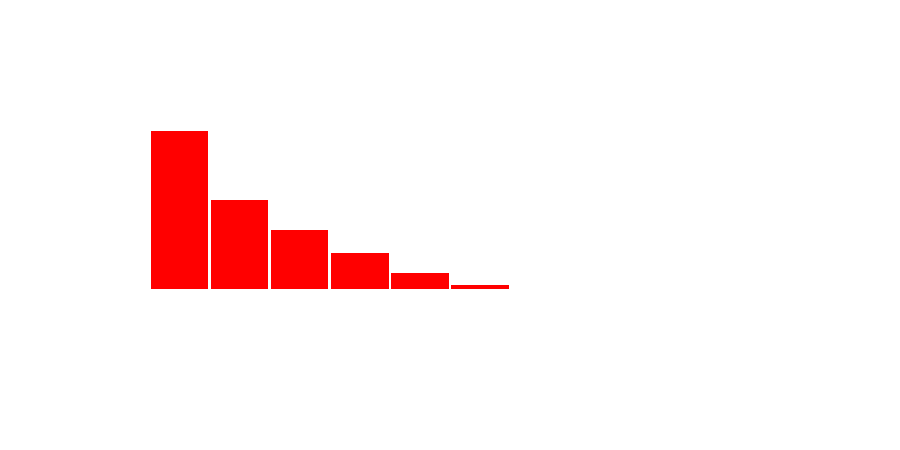
\includegraphics[scale = 0.08, clip = true, trim= 50px 70px 50px 60px]{hist-31b77719e3773ad7ac2073785de62a5f.pdf} \\ 
  with\_exception & All issues featuring an exception. & 0.00 & 3.21 & 0.00 & 6.00 & 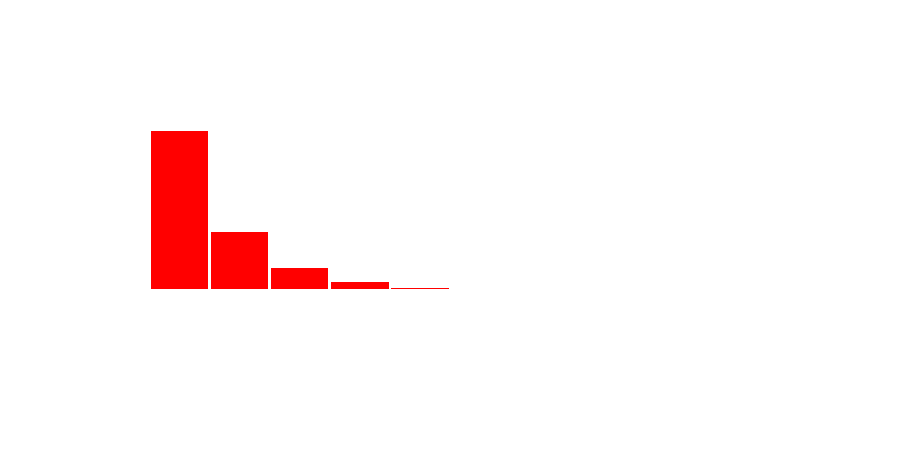
\includegraphics[scale = 0.08, clip = true, trim= 50px 70px 50px 60px]{hist-0c1305fc40f695dbdd1f4696db24f147.pdf} \\ 
  with\_stack & All issues featuring a stack trace. & 0.00 & 2.67 & 0.00 & 4.00 & 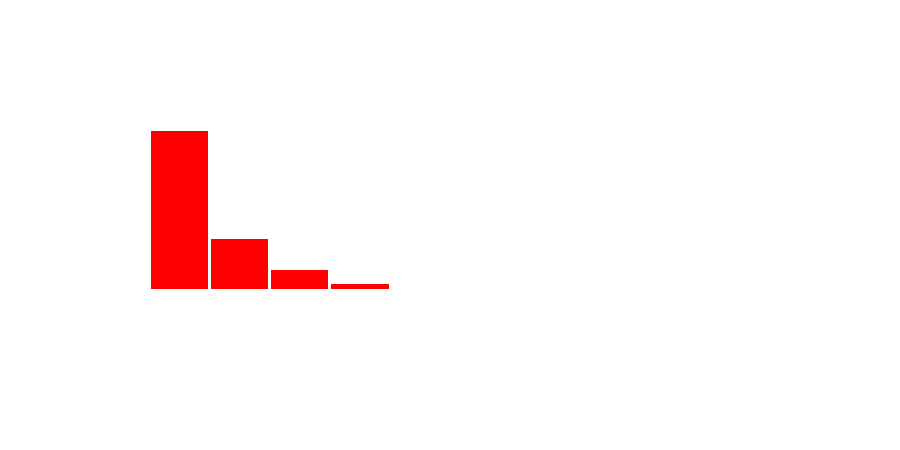
\includegraphics[scale = 0.08, clip = true, trim= 50px 70px 50px 60px]{hist-896524802e915aa3f01ef1ecd2489e7e.pdf} \\ 
  defect\_issues & All issues labeled as defect. & 0.00 & 5.51 & 0.00 & 12.00 & 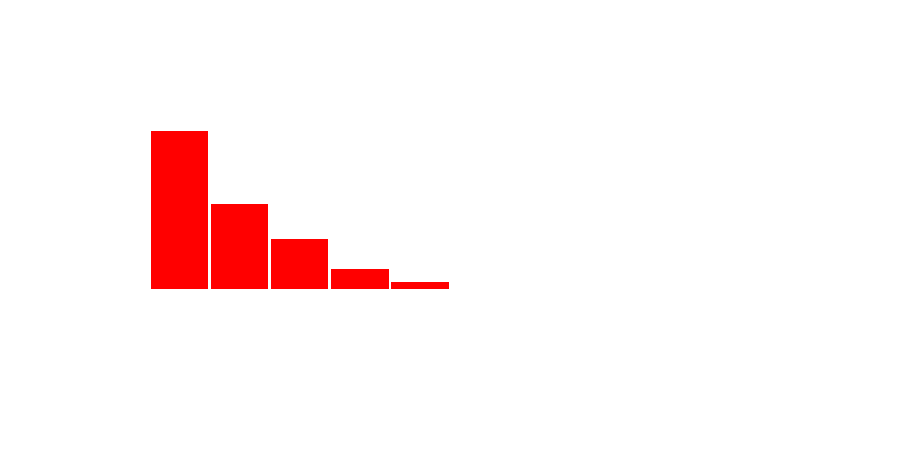
\includegraphics[scale = 0.08, clip = true, trim= 50px 70px 50px 60px]{hist-5d0ab95cd3e300c21b0a40d6bec58e4c.pdf} \\ 
  defect\_with\_exception & All issues labeled labeled as defect and including an exception. & 0.00 & 1.82 & 0.00 & 1.00 & 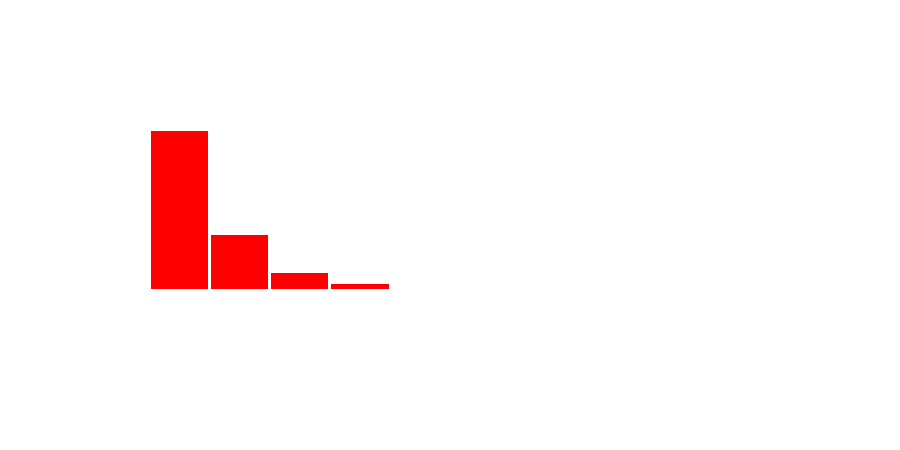
\includegraphics[scale = 0.08, clip = true, trim= 50px 70px 50px 60px]{hist-502028d1a7e2e77414e2f9f63e0bcd50.pdf} \\ 
  defect\_with\_stack & All issues labeled labeled as defect and including a stacktrace & 0.00 & 1.73 & 0.00 & 1.00 & 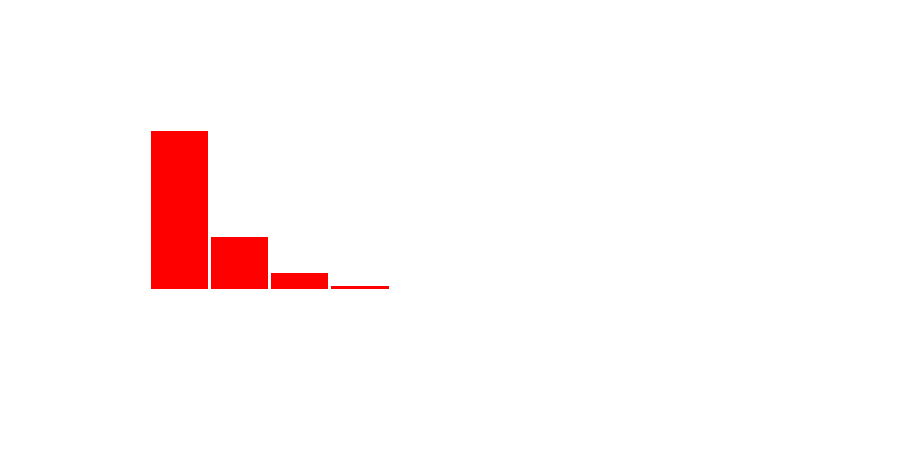
\includegraphics[scale = 0.08, clip = true, trim= 50px 70px 50px 60px]{hist-dab0764147debd99066c84814d46d50e.pdf} \\ 
   \hline
   \multicolumn{2}{l}{\bfseries{Android}}\\
   all & All issues recorded for the project. & 2.00 & 67.70 & 20.00 & 248.00 & 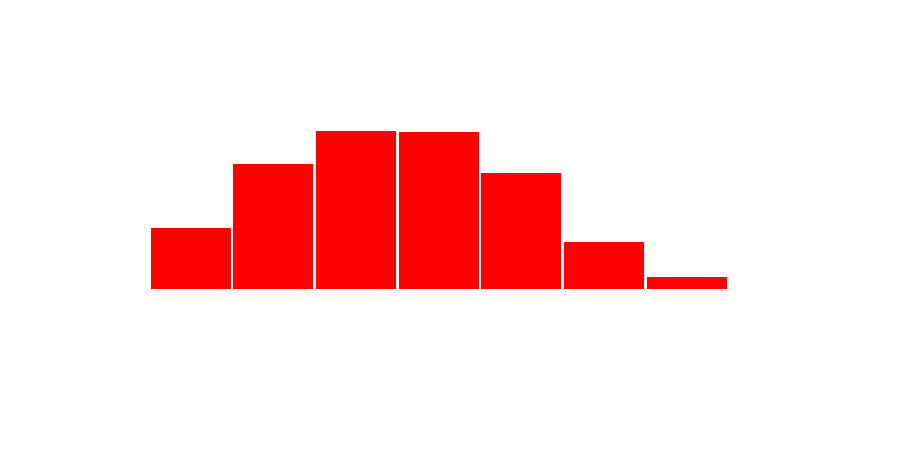
\includegraphics[scale = 0.08, clip = true, trim= 50px 70px 50px 60px]{hist-5d4a87daa44c63097df9bb1f3506d541.pdf} \\ 
  with\_exception & All issues featuring an exception. & 1.00 & 8.16 & 2.00 & 34.00 & 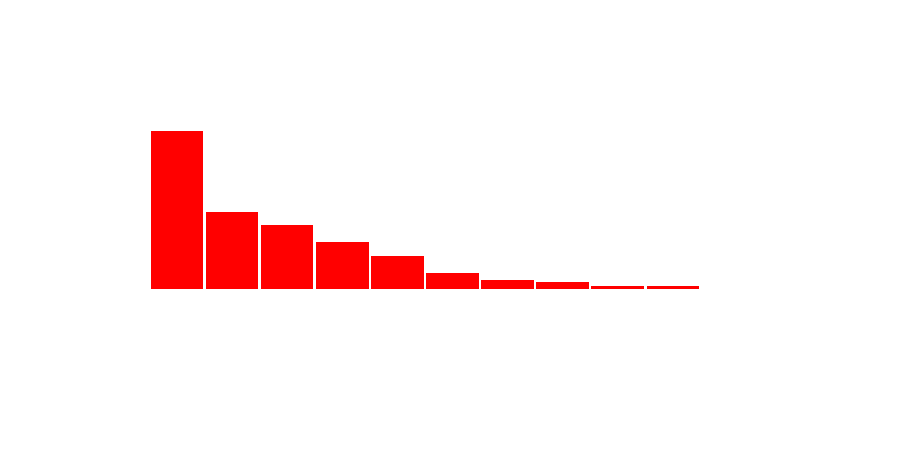
\includegraphics[scale = 0.08, clip = true, trim= 50px 70px 50px 60px]{hist-bf73235d0503f937ef6f36c28cf1ba0d.pdf} \\ 
  with\_stack & All issues featuring a stack trace. & 1.00 & 6.44 & 2.00 & 27.00 & 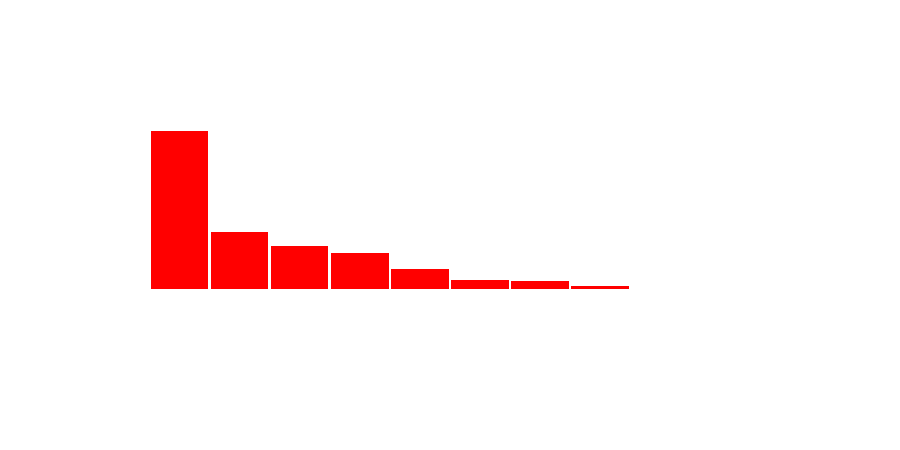
\includegraphics[scale = 0.08, clip = true, trim= 50px 70px 50px 60px]{hist-528cb6be67074e6e2c22d11245920e13.pdf} \\ 
  defect\_issues & All issues labeled as defect. & 0.00 & 13.28 & 1.00 & 52.00 & 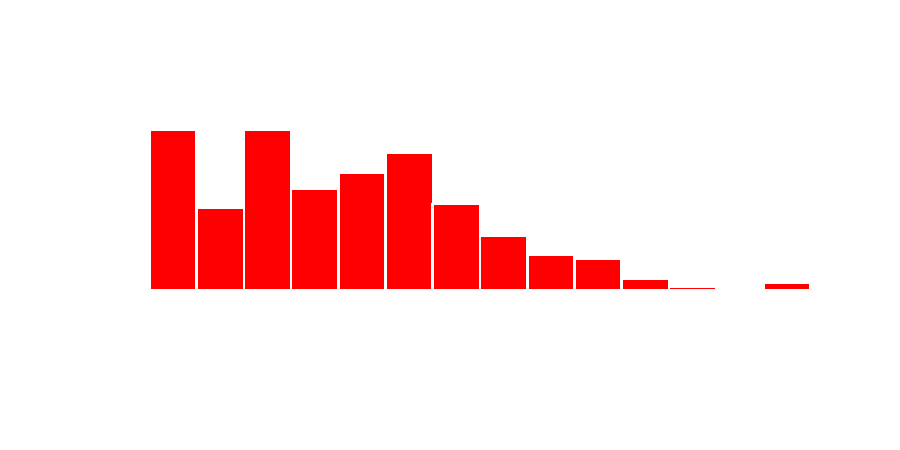
\includegraphics[scale = 0.08, clip = true, trim= 50px 70px 50px 60px]{hist-eb1797e86ef23b2a07907e5ccbeff7b9.pdf} \\ 
  defect\_with\_exception & All issues labeled labeled as defect and including an exception. & 0.00 & 3.25 & 0.00 & 13.00 & 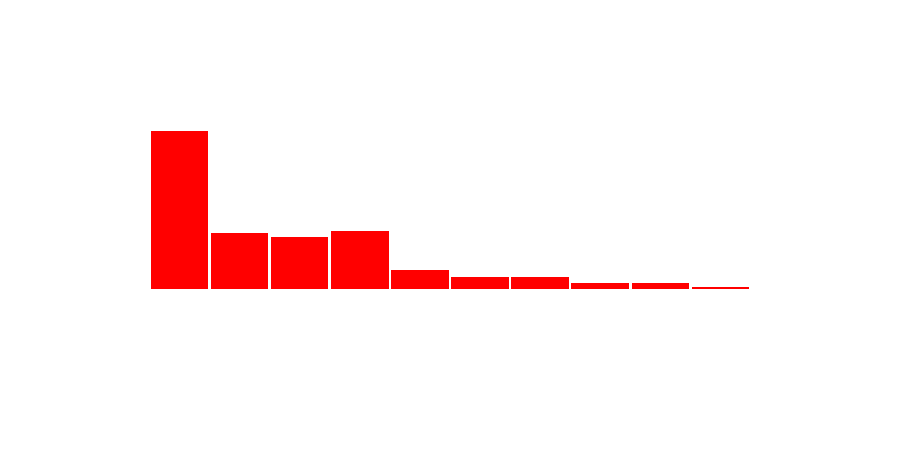
\includegraphics[scale = 0.08, clip = true, trim= 50px 70px 50px 60px]{hist-f1a879616aa3e0995db35c6c02bc8520.pdf} \\ 
  defect\_with\_stack & All issues labeled labeled as defect and including a stacktrace & 0.00 & 2.92 & 0.00 & 10.00 & 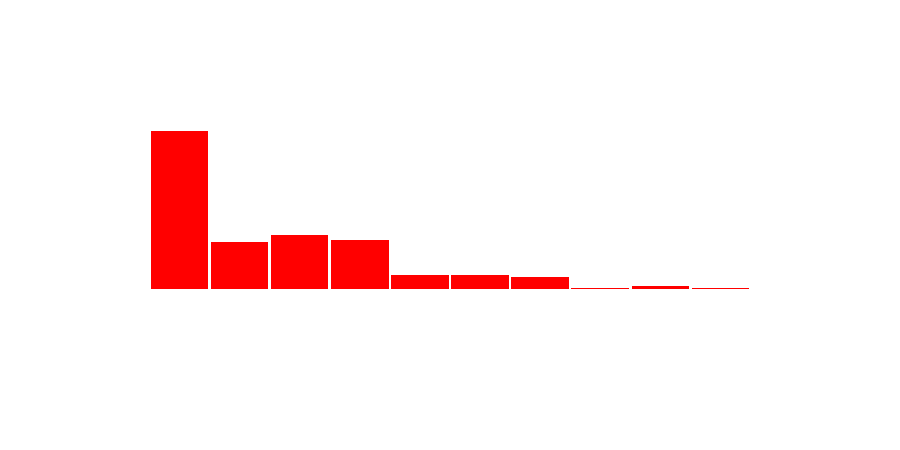
\includegraphics[scale = 0.08, clip = true, trim= 50px 70px 50px 60px]{hist-49dbfa02c366cab8b489f33014de587d.pdf} \\
 \hline
 \end{tabular}
\caption{Descriptive statistics for the analyzed issue dataset. Historgrams are in log scale.} 
\label{tab:stacktrace-stats}
\end{table*}
